\chapter{Lehrauftrag}
\label{lehrauftrag}
\info{Definition: Der Lehrauftrag enth�lt die Stunden, die von einem Lektor im Laufe des kommenden Semesters gehalten werden m�ssen (inklusive Betreuungen). Der Lehrauftrag wird den Lektoren vor Beginn des Semesters zur Unterschrift vorgelegt.}\\
\section{Erstellen eines Lehrauftrags}
\underline{Lehrauftrag f�r einen Lektor:}\\Im Tab Lektor Studiengang und Lektor ausw�hlen und rechts auf Lehrauftrag klicken.\\ \\
\underline{Lehrauftrag f�r alle Lektoren eines Studiengangs:}\\Studiengang ausw�hlen und im Men�punkt \textbf{Berichte -  Lehrauftr�ge} klicken.\\ \\
\underline{Lehrauftrag f�r eine Firma erstellen:}\\
Es besteht die M�glichkeit den Lehrauftrag auf den Namen einer Firma auszustellen.\\ \\
Folgende Schritte sind dazu n�tig:
\begin{itemize}
	\item Die Firma unter \textbf{Extras - Firmenverwaltung} anlegen.
	\item Beim Lektor wird unter \textbf{Kontakt} eine neue Adresse angelegt(siehe \ref{kontakte}):
	\begin{itemize}
	 	\item Diese Adresse ist die Firmenadresse, an die der Lehrauftrag gesendet wird.
	 	\item Die Adresse muss als Zustelladresse markiert sein.
	 	\item Im Feld Firma muss die Firma ausgew�hlt werden.
	\end{itemize}
\end{itemize}
\begin{figure}
	\centering
	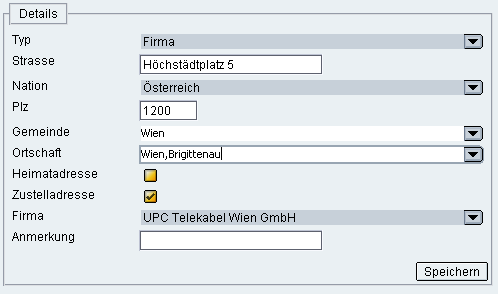
\includegraphics[width=0.75\textwidth]{FAS_Kontakte_Firma.png}
	\caption{Firmenkontakte}
	\label{firmenkontakt}
\end{figure}
\achtung{\textbf{Wichtig} Eine Lehrveranstaltung scheint nur am Lehrauftrag auf, wenn eine Gruppe zugeteilt ist!}\\
\\
Um alle Lehrauftr�ge eines bestimmten Lektors anzuzeigen k�nnen Sie den Lektor ausw�hlen und den Men�punkt Berichte->Lehre->LV-Planung->Excel/HTML w�hlen.
